\section{Methodology}
After taking a quick look at the stereoscopic depth camera's inner workings, this
report details the capturing and aligning of point clouds for model reconstruction.
This process consists of a few steps:

 \begin{itemize}
   \item the use of the RealSense SDK and Viewer to produce depth images and point clouds \cite{librealsense},
   \item the use of MeshLab's registration (or align) methods to merge point clouds,
   \item a survey of some techniques available for smoothing, eliminating noise, and
   \item reconstructing a mesh from the merged point clouds.
 \end{itemize}


 \subsection{Depth Cameras and Depth Images}
  The workings of the previous generation of RealSense cameras are detailed in \cite{keselman2017intel}.
 The algorithm described therein has not significantly changed (I believe) in the 400 series.
 The new features seem to be additional on-device hardware post-processing.

 These cameras produce four-channel image composed of the standard RGB colour channels together with a fourth depth channel. The depth channel associates to each pixel an estimate of the distance from the camera to the surface.

 The D435 (and similar devices) use a stereoscopic technique inspired by human
 binocular vision.

 \begin{figure}[H]
  \centering
  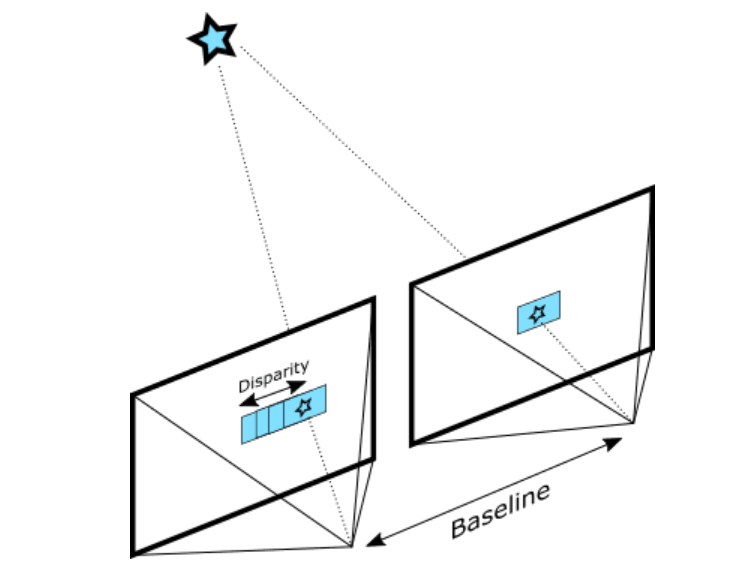
\includegraphics[width=0.45\textwidth]{binocular_vision.png}
  \caption{Binocular Vision}
  \end{figure}

 It is possible to compute a pixel's depth by comparing the images produced by two cameras placed at known distances and pointing in generally the same direction. After projecting the images onto a common plane (the cameras produce images which are slightly ``angled''), the camera computes the \textit{disparity}
  $d$ between the two images.


 Disparity is the distance (in pixels) of a cluster of pixels from one image to the other.
 Objects closer to the camera will have greater disparity between the two images, distant
 objects less so.
 With distance $B$ between the two cameras and the focal length $f$, the disparity allows the camera
 to infer the depth $z$ using the formula:

 \[ z = \frac{f \cdot B}{d} \]

 However, this simple stereoscopic approach struggles in many different
 environments. When materials are transparent, reflective, patterned, occluded or
 even brightly lit there may not be recognizable clusters to compare.
 To improve the robustness of the depth calculation on a variety
 of textures and surfaces, the devices additionally include an infrared projector.

 \begin{figure}[h]
 \centering
 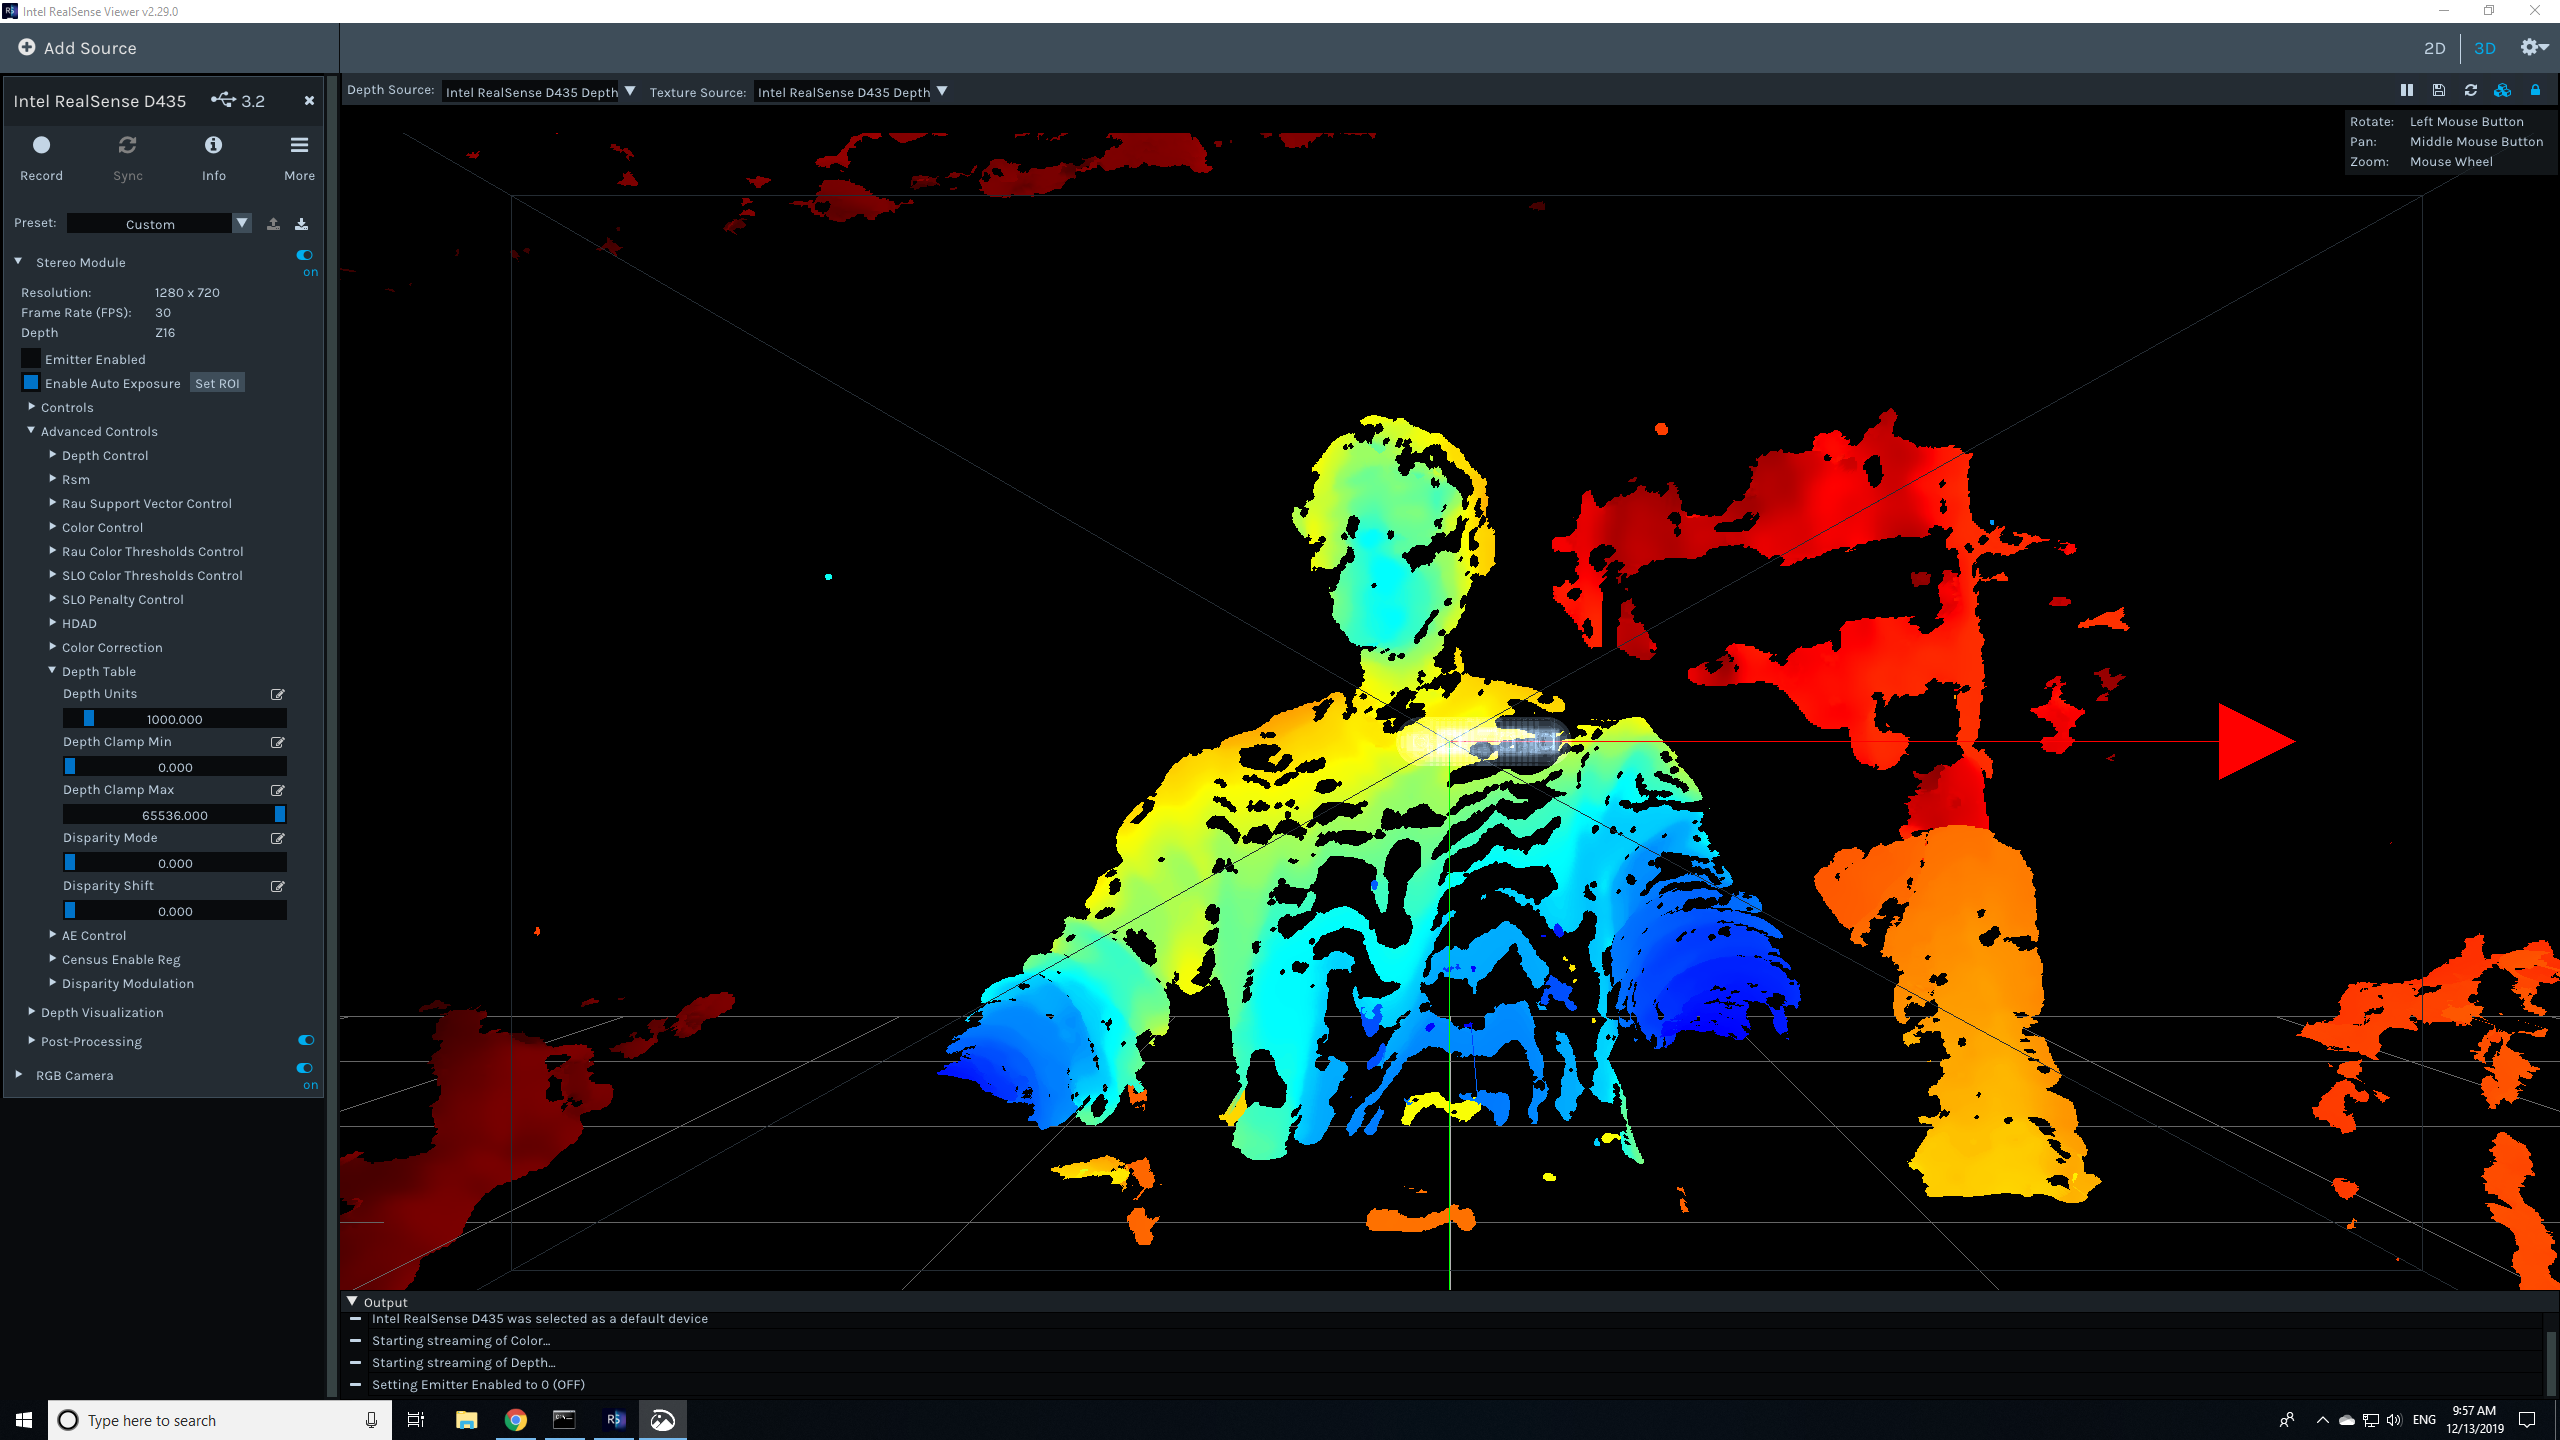
\includegraphics[width=0.35\textwidth]{without_emitter.png}
 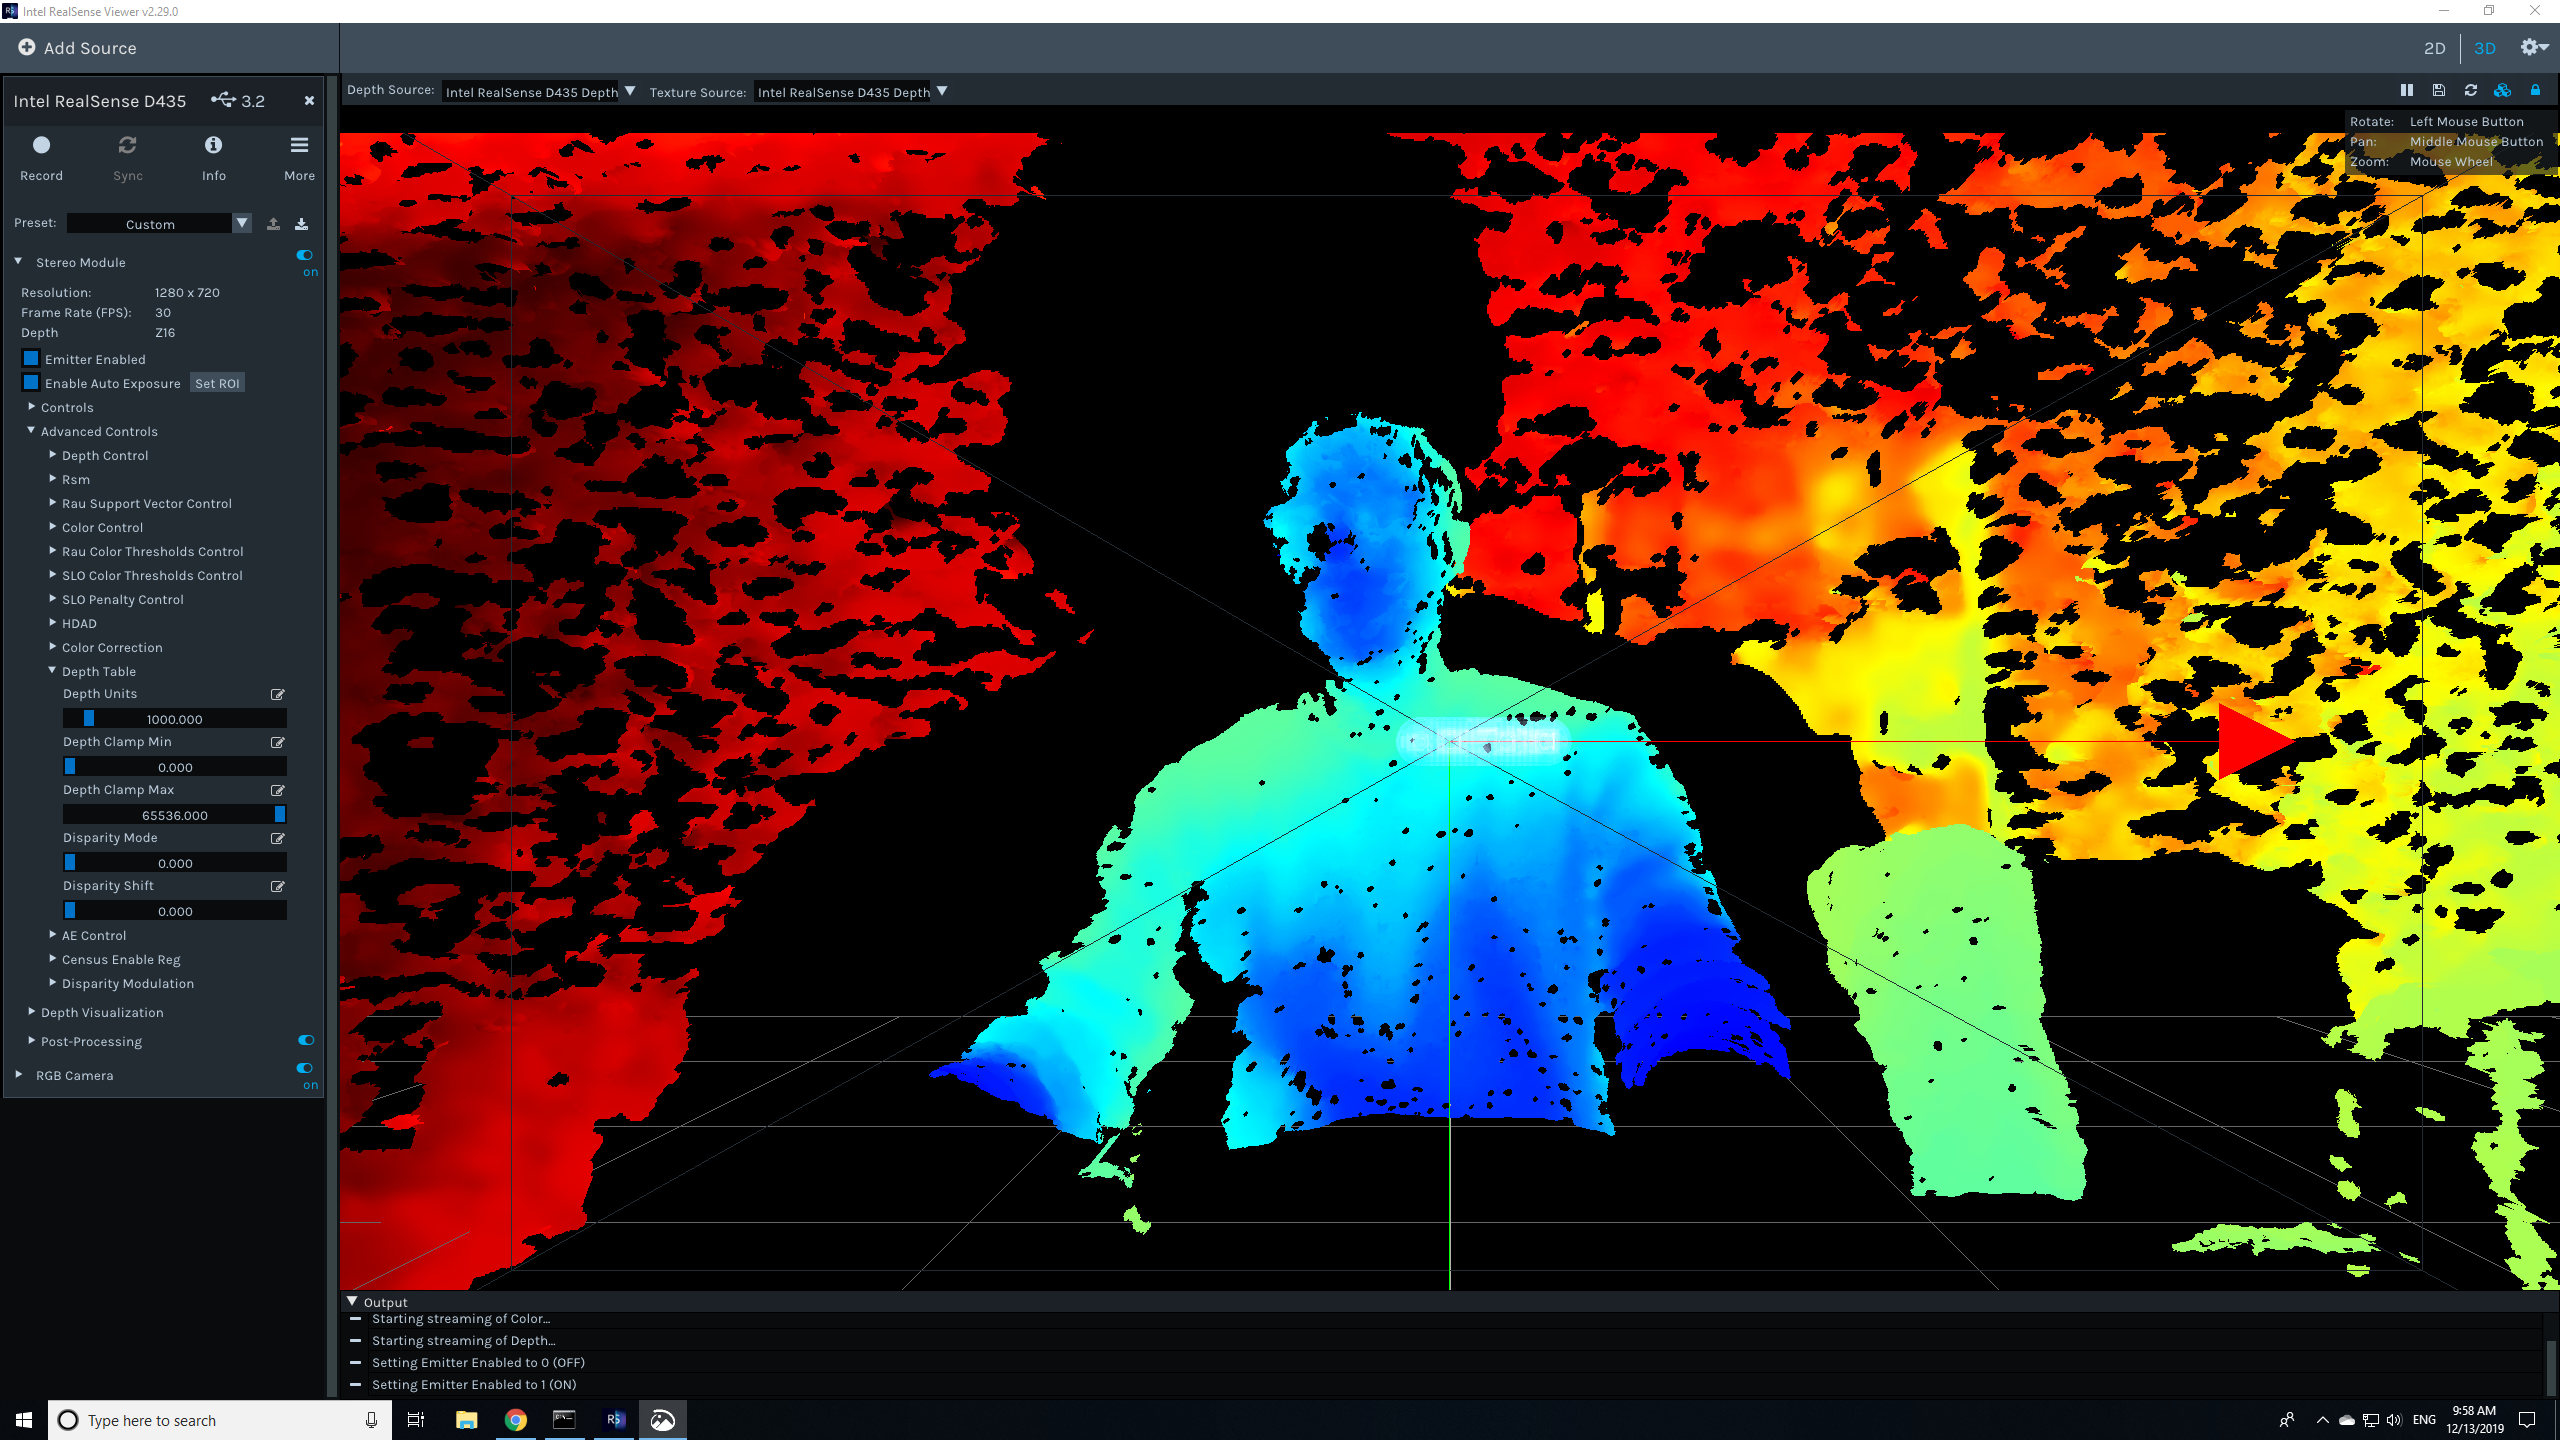
\includegraphics[width=0.35\textwidth]{with_emitter.png}
 \caption{Infrared emitter off (left) and on (right)}
 \end{figure}

 In the pictures above, you can see that without the emitter, the camera is
 unable to detect the uniformly white wall behind me. My sweater is also dotted with
 holes. The emitter seems to improve the robustness but  the unstructured infrared light
 seems to add a rippling distortion.

 All of the complexity of these calculations, of course, are abstracted in the Viewer
 and SDK bundled with the camera.
 Using the Intel software, it is straightforward to take depth-snapshots or videos
 and export them to mesh files.

 \subsection{Depth Pixel to Point Cloud Transformation}
 With the $x$ and $y$ coordinates of a pixel and a corresponding depth measurement $z$,
 it is possible to apply a transformation to obtain a point in a 3d frame of
 reference, say, ``in front of the camera''.

 This transformation depends on the configuration and specifications of the camera(s).
 Note that this conversion may involve a tradeoff. Each pixel's frustum is a thin but expanding shape so closer pixels are smaller than distant ones. Sophisticated transformations take this into consideration when converting depth values into voxels or points.

 It may be of interest that the RealSense SDK offers a CUDA implementation at:

 \url{github.com/IntelRealSense/librealsense/blob/master/src/cuda/cuda-pointcloud.cu}

 This version runs the per-pixel conversion on the GPU. The \textit{device} function
 performs the per-point computation and the \textit{global} function
 can be used to run a calculation on the GPU after allocating memory on the graphics device and
 defining the number of cores/thread blocks to use. Both share an \textit{intrisic} object which stores the specifications of the camera and current frame.
